
\begin{frame}
    \frametitle{Exercise 3.4 - 16}
    \textit{Problem Statement}\\
    Give an example of a topological space which is Hausdorff but not
    metrizable.
\end{frame}

\begin{frame}
    \frametitle{Examining the problem}

    We just proved Metrizable \(\Leftrightarrow\) Hausdorff, so what gives?
    \pause
    There is something quite important we used to establish all the ideas in
    that problem. 
    \pause
    \emph{Finiteness.} \pause In particular for the context of this problem,
    call it \emph{first countability}\pause, to be able to list the elements of
    the set in question finitely. % This will become important later.

\end{frame}

\begin{frame}
    \frametitle{Morphing Relationships}
    \centering
    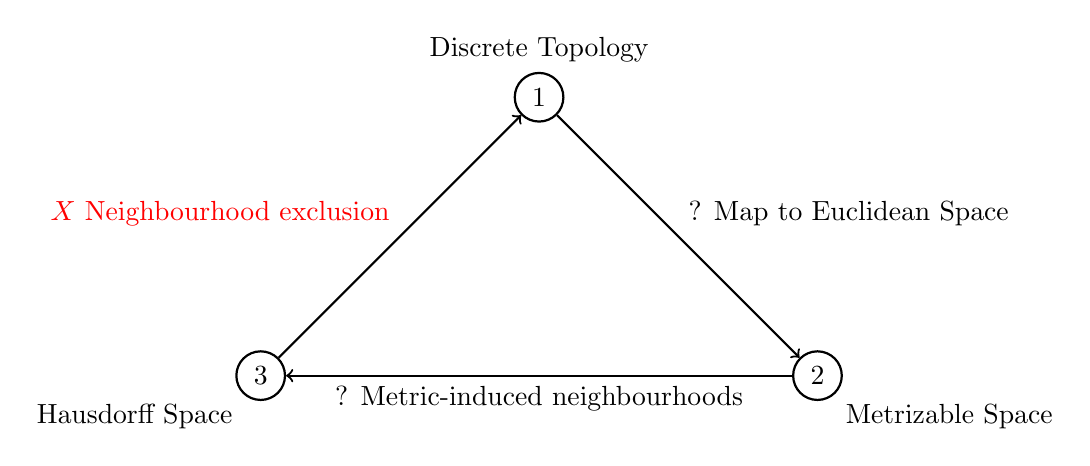
\begin{tikzpicture}[node distance={5cm}, thick, main/.style = {draw, circle}]
        \node[main, label=above:Discrete Topology] (1)                      {\(1\)};
        \node[main, label=below right:Metrizable Space] (2) [below right of=1]    {\(2\)};
        \node[main, label=below left:Hausdorff Space] (3) [below left of=1]      {\(3\)};

        % \pause

        \draw[->] (1) -- node[midway, above right] {? Map to Euclidean Space} (2);
        \draw[->] (2) -- node[midway, below] {? Metric-induced neighbourhoods} (3);
        \draw[->] (3) -- node[midway, above left] {\textcolor{red}{\(X\) Neighbourhood exclusion}} (1);

    \end{tikzpicture}

\end{frame}

\begin{frame}
    \frametitle{Chasing Broken Bridges}

    % infinite countable discrete space
    \begin{figure}
        \scalebox{1.4}{\input{fig/sankalp/countable_metrizable.pdf_tex}}
    \end{figure}

    % subset of euclidean space still

    \pause

    \begin{center}
        \emph{Still Metrizable!}
    \end{center}

\end{frame}

\begin{frame}
    \frametitle{Morphing Relationships}
    \centering
    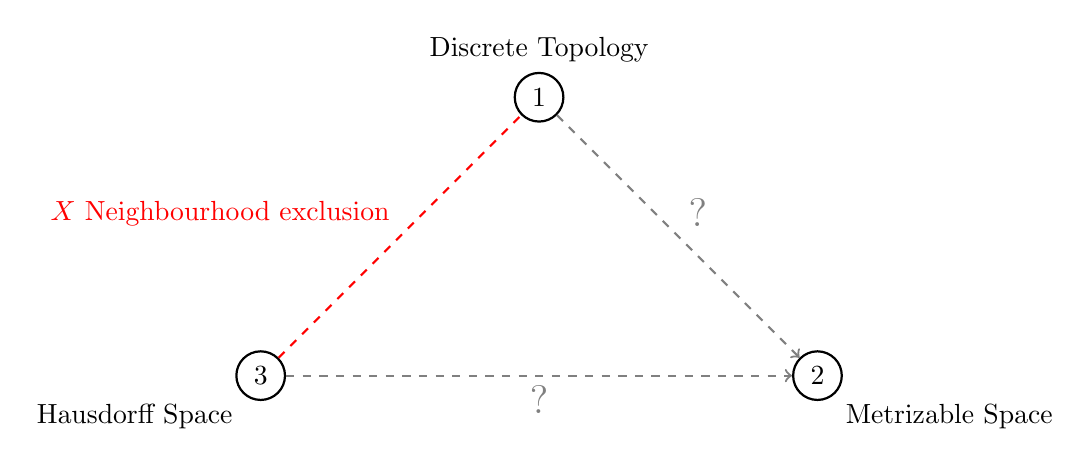
\begin{tikzpicture}[node distance={5cm}, thick, main/.style = {draw, circle}]
        \node[main, label=above:Discrete Topology] (1)                      {\(1\)};
        \node[main, label=below right:Metrizable Space] (2) [below right of=1]    {\(2\)};
        \node[main, label=below left:Hausdorff Space] (3) [below left of=1]      {\(3\)};

        % \pause

        \draw[->, color=gray] (1) -- node[midway, above right] {\Large ?} (2) [dashed];
        \draw[->, color=gray] (3) -- node[midway, below] {\Large ?} (2) [dashed];
        \draw[color=red] (3) -- node[midway, above left] {\textcolor{red}{\(X\) Neighbourhood exclusion}}(1) [dashed];

    \end{tikzpicture}

    \pause

    \begin{center}
        We have lost some information about the internal relationships while
        breaking one edge. \pause If finiteness doesn't break things enough,
        what did we use that might?
        % So our diagram order was chosen carefully to be annoying
    \end{center}

\end{frame}

\begin{frame}
    \frametitle{Countability}

    We broke our `weakest link' by removing the assumption of being able to
    finitely count the set, \emph{first countability}.\pause The next step is to
    remove the assumption that we are able to \emph{count at all}.\pause This is
    second countability.

    \pause

    In fact, every second countable Hausdorff space is metrizable.
    % The discreteness was a ruse all along

\end{frame}

\begin{frame}
    \frametitle{Shepherd's Nightmare}

    Combining everything, consider the space

    \begin{gather*}
        (\topx, \tau) \in \catTop\\
        \topx \textnormal{ is not second-countable}\\
        \forall x \in \topx \; x \in \tau \textnormal{ (discrete topology)}
    \end{gather*}

\end{frame}

\begin{frame}
    \frametitle{Shepherd's Nightmare}

    As a visual example, consider \(\reals^2\) with the discrete topology.
    \pause If a metric existed on this space, 

\end{frame}